% ARTICLE ----
% This is just here so I know exactly what I'm looking at in Rstudio when messing with stuff.
\documentclass[11pt,]{article}
\usepackage[left=1in,top=1in,right=1in,bottom=1in]{geometry}
\newcommand*{\authorfont}{\fontfamily{phv}\selectfont}
\usepackage[]{mathpazo}


  \usepackage[T1]{fontenc}
  \usepackage[utf8]{inputenc}




\usepackage{abstract}
\renewcommand{\abstractname}{}    % clear the title
\renewcommand{\absnamepos}{empty} % originally center

\renewenvironment{abstract}
 {{%
    \setlength{\leftmargin}{0mm}
    \setlength{\rightmargin}{\leftmargin}%
  }%
  \relax}
 {\endlist}

\makeatletter
\def\@maketitle{%
  \newpage
%  \null
%  \vskip 2em%
%  \begin{center}%
  \let \footnote \thanks
    {\fontsize{18}{20}\selectfont\raggedright  \setlength{\parindent}{0pt} \@title \par}%
}
%\fi
\makeatother




\setcounter{secnumdepth}{0}

\usepackage{color}
\usepackage{fancyvrb}
\newcommand{\VerbBar}{|}
\newcommand{\VERB}{\Verb[commandchars=\\\{\}]}
\DefineVerbatimEnvironment{Highlighting}{Verbatim}{commandchars=\\\{\}}
% Add ',fontsize=\small' for more characters per line
\usepackage{framed}
\definecolor{shadecolor}{RGB}{248,248,248}
\newenvironment{Shaded}{\begin{snugshade}}{\end{snugshade}}
\newcommand{\AlertTok}[1]{\textcolor[rgb]{0.94,0.16,0.16}{#1}}
\newcommand{\AnnotationTok}[1]{\textcolor[rgb]{0.56,0.35,0.01}{\textbf{\textit{#1}}}}
\newcommand{\AttributeTok}[1]{\textcolor[rgb]{0.13,0.29,0.53}{#1}}
\newcommand{\BaseNTok}[1]{\textcolor[rgb]{0.00,0.00,0.81}{#1}}
\newcommand{\BuiltInTok}[1]{#1}
\newcommand{\CharTok}[1]{\textcolor[rgb]{0.31,0.60,0.02}{#1}}
\newcommand{\CommentTok}[1]{\textcolor[rgb]{0.56,0.35,0.01}{\textit{#1}}}
\newcommand{\CommentVarTok}[1]{\textcolor[rgb]{0.56,0.35,0.01}{\textbf{\textit{#1}}}}
\newcommand{\ConstantTok}[1]{\textcolor[rgb]{0.56,0.35,0.01}{#1}}
\newcommand{\ControlFlowTok}[1]{\textcolor[rgb]{0.13,0.29,0.53}{\textbf{#1}}}
\newcommand{\DataTypeTok}[1]{\textcolor[rgb]{0.13,0.29,0.53}{#1}}
\newcommand{\DecValTok}[1]{\textcolor[rgb]{0.00,0.00,0.81}{#1}}
\newcommand{\DocumentationTok}[1]{\textcolor[rgb]{0.56,0.35,0.01}{\textbf{\textit{#1}}}}
\newcommand{\ErrorTok}[1]{\textcolor[rgb]{0.64,0.00,0.00}{\textbf{#1}}}
\newcommand{\ExtensionTok}[1]{#1}
\newcommand{\FloatTok}[1]{\textcolor[rgb]{0.00,0.00,0.81}{#1}}
\newcommand{\FunctionTok}[1]{\textcolor[rgb]{0.13,0.29,0.53}{\textbf{#1}}}
\newcommand{\ImportTok}[1]{#1}
\newcommand{\InformationTok}[1]{\textcolor[rgb]{0.56,0.35,0.01}{\textbf{\textit{#1}}}}
\newcommand{\KeywordTok}[1]{\textcolor[rgb]{0.13,0.29,0.53}{\textbf{#1}}}
\newcommand{\NormalTok}[1]{#1}
\newcommand{\OperatorTok}[1]{\textcolor[rgb]{0.81,0.36,0.00}{\textbf{#1}}}
\newcommand{\OtherTok}[1]{\textcolor[rgb]{0.56,0.35,0.01}{#1}}
\newcommand{\PreprocessorTok}[1]{\textcolor[rgb]{0.56,0.35,0.01}{\textit{#1}}}
\newcommand{\RegionMarkerTok}[1]{#1}
\newcommand{\SpecialCharTok}[1]{\textcolor[rgb]{0.81,0.36,0.00}{\textbf{#1}}}
\newcommand{\SpecialStringTok}[1]{\textcolor[rgb]{0.31,0.60,0.02}{#1}}
\newcommand{\StringTok}[1]{\textcolor[rgb]{0.31,0.60,0.02}{#1}}
\newcommand{\VariableTok}[1]{\textcolor[rgb]{0.00,0.00,0.00}{#1}}
\newcommand{\VerbatimStringTok}[1]{\textcolor[rgb]{0.31,0.60,0.02}{#1}}
\newcommand{\WarningTok}[1]{\textcolor[rgb]{0.56,0.35,0.01}{\textbf{\textit{#1}}}}
\usepackage{longtable,booktabs}

% --------------------------------
% Separating this because this no
% longer works as of pandoc 3.2.1
% -------------------------------
%%\usepackage{graphicx,grffile}
%\makeatletter
%\def\maxwidth{\ifdim\Gin@nat@width>\linewidth\linewidth\else\Gin@nat@width\fi}
%\def\maxheight{\ifdim\Gin@nat@height>\textheight\textheight\else\Gin@nat@height\fi}
%\makeatother
%% Scale images if necessary, so that they will not overflow the page
%% margins by default, and it is still possible to overwrite the defaults
%% using explicit options in \includegraphics[width, height, ...]{}
%\setkeys{Gin}{width=\maxwidth,height=\maxheight,keepaspectratio}
%
% ---------------------------------
% This works now: HT: Justin Esarey
% ---------------------------------
\usepackage{graphicx}
\makeatletter
\newsavebox\pandoc@box
\newcommand*\pandocbounded[1]{% scales image to fit in text height/width
  \sbox\pandoc@box{#1}%
  \Gscale@div\@tempa{\textheight}{\dimexpr\ht\pandoc@box+\dp\pandoc@box\relax}%
  \Gscale@div\@tempb{\linewidth}{\wd\pandoc@box}%
  \ifdim\@tempb\p@<\@tempa\p@\let\@tempa\@tempb\fi% select the smaller of both
  \ifdim\@tempa\p@<\p@\scalebox{\@tempa}{\usebox\pandoc@box}%
  \else\usebox{\pandoc@box}%
  \fi%
}
% Set default figure placement to htbp
\def\fps@figure{htbp}
\makeatother

% ^ saving this note in case I want some kind of conditional operation thingie.


\title{Simulação do Brasileirão 2026  }



\author{\Large Caio Gomes
Alves\vspace{0.05in} \newline\normalsize\emph{Instituto de Matemática,
Estatística e Computação Científica - UNICAMP}  }


\date{}

\usepackage{titlesec}

\titleformat*{\section}{\normalsize\bfseries}
\titleformat*{\subsection}{\normalsize\itshape}
\titleformat*{\subsubsection}{\normalsize\itshape}
\titleformat*{\paragraph}{\normalsize\itshape}
\titleformat*{\subparagraph}{\normalsize\itshape}





\newtheorem{hypothesis}{Hypothesis}
\usepackage{setspace}


% set default figure placement to htbp
\makeatletter
\def\fps@figure{htbp}
\makeatother


% move the hyperref stuff down here, after header-includes, to allow for - \usepackage{hyperref}

\makeatletter
\@ifpackageloaded{hyperref}{}{%
\ifxetex
  \PassOptionsToPackage{hyphens}{url}\usepackage[setpagesize=false, % page size defined by xetex
              unicode=false, % unicode breaks when used with xetex
              xetex]{hyperref}
\else
  \PassOptionsToPackage{hyphens}{url}\usepackage[draft,unicode=true]{hyperref}
\fi
}

\@ifpackageloaded{color}{
    \PassOptionsToPackage{usenames,dvipsnames}{color}
}{%
    \usepackage[usenames,dvipsnames]{color}
}
\makeatother
\hypersetup{breaklinks=true,
            bookmarks=true,
            pdfauthor={Caio Gomes Alves (Instituto de Matemática,
Estatística e Computação Científica - UNICAMP)},
             pdfkeywords = {},
            pdftitle={Simulação do Brasileirão 2026},
            colorlinks=true,
            citecolor=blue,
            urlcolor=blue,
            linkcolor=magenta,
            pdfborder={0 0 0}}
\urlstyle{same}  % don't use monospace font for urls

% Add an option for endnotes. -----


% add tightlist ----------
\providecommand{\tightlist}{%
\setlength{\itemsep}{0pt}\setlength{\parskip}{0pt}}

% add some other packages ----------

% \usepackage{multicol}
% This should regulate where figures float
% See: https://tex.stackexchange.com/questions/2275/keeping-tables-figures-close-to-where-they-are-mentioned
\usepackage[section]{placeins}

% CSL environment change -----


% Last minute stuff -----
\usepackage{amssymb,amsmath} % HT @ashenkin


\begin{document}

% \pagenumbering{arabic}% resets `page` counter to 1
%
% \maketitle

{% \usefont{T1}{pnc}{m}{n}
\setlength{\parindent}{0pt}
\thispagestyle{plain}
{\fontsize{18}{20}\selectfont\raggedright
\maketitle  % title \par

}

{
   \vskip 13.5pt\relax \normalsize\fontsize{11}{12}
\textbf{\authorfont Caio Gomes Alves} \hskip 15pt \emph{\small Instituto
de Matemática, Estatística e Computação Científica - UNICAMP}   

}

}






\vskip -8.5pt


 % removetitleabstract

\noindent 

\hypertarget{simulauxe7uxe3o-do-campeonato}{%
\section{Simulação do Campeonato}\label{simulauxe7uxe3o-do-campeonato}}

\hypertarget{construuxe7uxe3o-da-tabela}{%
\subsection{Construção da tabela}\label{construuxe7uxe3o-da-tabela}}

Para a simulação, vejamos primeiro como se comportam os valores de
\(\theta\) e \(\phi\) para cada um dos times:

\begin{Shaded}
\begin{Highlighting}[]
\NormalTok{dados\_bras }\OtherTok{\textless{}{-}} \FunctionTok{read.csv}\NormalTok{(}\StringTok{"\textasciitilde{}/Downloads/brasileirao\_2026.csv"}\NormalTok{)}

\CommentTok{\# Criando as taxas theta e phi:}
\NormalTok{taxas\_estimadas }\OtherTok{\textless{}{-}} \FunctionTok{left\_join}\NormalTok{(}
    \CommentTok{\# Taxas dos mandantes:}
\NormalTok{    (dados\_bras }\SpecialCharTok{\%\textgreater{}\%}
    \FunctionTok{mutate}\NormalTok{(}\AttributeTok{time =}\NormalTok{ time\_mandante) }\SpecialCharTok{\%\textgreater{}\%}
    \FunctionTok{group\_by}\NormalTok{(time) }\SpecialCharTok{\%\textgreater{}\%}
    \FunctionTok{summarise}\NormalTok{(}\AttributeTok{theta\_m =} \FunctionTok{mean}\NormalTok{(gols\_mandante, }\AttributeTok{na.rm =}\NormalTok{ T),}
              \AttributeTok{phi\_v =} \FunctionTok{mean}\NormalTok{(gols\_visitante, }\AttributeTok{na.rm =}\NormalTok{ T))),}
    \CommentTok{\# Taxas dos visitantes:}
\NormalTok{    (dados\_bras }\SpecialCharTok{\%\textgreater{}\%}
    \FunctionTok{mutate}\NormalTok{(}\AttributeTok{time =}\NormalTok{ time\_visitante) }\SpecialCharTok{\%\textgreater{}\%}
    \FunctionTok{group\_by}\NormalTok{(time) }\SpecialCharTok{\%\textgreater{}\%}
    \FunctionTok{summarise}\NormalTok{(}\AttributeTok{theta\_v =} \FunctionTok{mean}\NormalTok{(gols\_visitante, }\AttributeTok{na.rm =}\NormalTok{ T),}
              \AttributeTok{phi\_m =} \FunctionTok{mean}\NormalTok{(gols\_mandante, }\AttributeTok{na.rm =}\NormalTok{ T))),}
    \CommentTok{\# Agrupa por time:}
    \AttributeTok{by =} \StringTok{"time"}\NormalTok{)}
\end{Highlighting}
\end{Shaded}

\begin{longtable}[]{@{}lrrrr@{}}
\toprule\noalign{}
Time & theta\_m & phi\_v & theta\_v & phi\_m \\
\midrule\noalign{}
\endhead
\bottomrule\noalign{}
\endlastfoot
Athletico-PR & 1.769231 & 0.7692308 & 1.1666667 & 1.2500000 \\
Atlético-MG & 1.727273 & 1.2727273 & 1.0000000 & 1.0769231 \\
Bahia & 1.538461 & 1.0000000 & 1.4166667 & 1.4166667 \\
Botafogo & 1.818182 & 1.5454545 & 1.3076923 & 1.7692308 \\
Bragantino & 1.416667 & 0.9166667 & 1.0000000 & 1.1666667 \\
Chapecoense & 1.416667 & 2.2500000 & 0.6666667 & 1.8333333 \\
Corinthians & 1.000000 & 0.8461538 & 1.0833333 & 1.1666667 \\
Coritiba & 1.250000 & 1.1666667 & 1.3846154 & 1.4615385 \\
Cruzeiro & 1.615385 & 1.1538462 & 1.1666667 & 1.7500000 \\
Flamengo & 2.000000 & 0.6666667 & 2.0000000 & 1.0000000 \\
Fluminense & 1.769231 & 1.0769231 & 1.3333333 & 1.5000000 \\
Grêmio & 1.750000 & 1.1666667 & 0.5000000 & 1.5000000 \\
Internacional & 1.076923 & 1.0000000 & 1.0000000 & 1.5000000 \\
Mirassol & 1.307692 & 1.4615385 & 0.8333333 & 1.6666667 \\
Palmeiras & 1.750000 & 0.7500000 & 1.8461538 & 0.9230769 \\
Remo & 1.416667 & 1.3333333 & 1.0000000 & 2.0000000 \\
Santos & 1.384615 & 1.3076923 & 1.4545455 & 1.7272727 \\
São Paulo & 1.636364 & 0.9090909 & 0.8461538 & 1.3846154 \\
Vasco & 1.230769 & 1.3846154 & 1.0000000 & 1.9090909 \\
Vitória & 1.333333 & 0.7500000 & 0.6153846 & 2.1538462 \\
\end{longtable}

Com isso, podemos criar uma função que adiciona os valores das taxas
calculadas em cada uma das linhas das rodadas do campeonato, criando um
data.frame aumentado, que será usado na simulação:

\begin{Shaded}
\begin{Highlighting}[]
\NormalTok{cria\_df\_taxas }\OtherTok{\textless{}{-}} \ControlFlowTok{function}\NormalTok{(df, taxas) \{}
\NormalTok{    times }\OtherTok{\textless{}{-}} \FunctionTok{unique}\NormalTok{(taxas}\SpecialCharTok{$}\NormalTok{time)}
\NormalTok{    df\_mandante }\OtherTok{\textless{}{-}} \FunctionTok{left\_join}\NormalTok{(df, (taxas }\SpecialCharTok{\%\textgreater{}\%}
                                  \FunctionTok{select}\NormalTok{(}\AttributeTok{time\_mandante =}\NormalTok{ time,}
\NormalTok{                                         theta\_m, phi\_m)), }\AttributeTok{by =} \StringTok{"time\_mandante"}\NormalTok{) }\SpecialCharTok{\%\textgreater{}\%}
        \FunctionTok{select}\NormalTok{(theta\_m, phi\_m)}
\NormalTok{    df\_visitante }\OtherTok{\textless{}{-}} \FunctionTok{left\_join}\NormalTok{(df, (taxas }\SpecialCharTok{\%\textgreater{}\%}
                                   \FunctionTok{select}\NormalTok{(}\AttributeTok{time\_visitante =}\NormalTok{ time,}
\NormalTok{                                          theta\_v, phi\_v)), }\AttributeTok{by =} \StringTok{"time\_visitante"}\NormalTok{) }\SpecialCharTok{\%\textgreater{}\%}
        \FunctionTok{select}\NormalTok{(theta\_v, phi\_v)}
\NormalTok{    df\_completo }\OtherTok{\textless{}{-}} \FunctionTok{cbind}\NormalTok{(df, df\_mandante, df\_visitante)}
    \FunctionTok{return}\NormalTok{(df\_completo)}
\NormalTok{\}}

\NormalTok{df\_completo }\OtherTok{\textless{}{-}} \FunctionTok{cria\_df\_taxas}\NormalTok{(dados\_bras, taxas\_estimadas)}
\end{Highlighting}
\end{Shaded}

Com o data.frame completo, separaremos em jogos realizados (que não
precisam passar por simulação) e jogos a realizar (que terão os placares
simulados usando os valores de \(\theta\) e \(\phi\) calculados
anteriormente):

\begin{Shaded}
\begin{Highlighting}[]
\NormalTok{jogos\_realizados }\OtherTok{\textless{}{-}}\NormalTok{ df\_completo }\SpecialCharTok{\%\textgreater{}\%} \FunctionTok{filter}\NormalTok{(}\SpecialCharTok{!}\FunctionTok{is.na}\NormalTok{(gols\_mandante))}
\NormalTok{jogos\_futuros }\OtherTok{\textless{}{-}}\NormalTok{ df\_completo }\SpecialCharTok{\%\textgreater{}\%} \FunctionTok{filter}\NormalTok{(}\FunctionTok{is.na}\NormalTok{(gols\_mandante))}
\end{Highlighting}
\end{Shaded}

A função que calcula a pontuação do campeonato deve considerar os casos
de vitória/empate/derrota, além de calcular os fatores de desempate
(número de vitórias, saldo de gols e quantidade de gols marcados):

\begin{Shaded}
\begin{Highlighting}[]
\NormalTok{calcula\_tabela }\OtherTok{\textless{}{-}} \ControlFlowTok{function}\NormalTok{(df) \{}
\NormalTok{    df }\SpecialCharTok{\%\textgreater{}\%}
        \FunctionTok{mutate}\NormalTok{(}
            \CommentTok{\# Pontos do mandante:}
            \AttributeTok{pts\_m =} \FunctionTok{case\_when}\NormalTok{(gols\_mandante }\SpecialCharTok{\textgreater{}}\NormalTok{ gols\_visitante }\SpecialCharTok{\textasciitilde{}} \DecValTok{3}\NormalTok{,}
\NormalTok{                              gols\_mandante }\SpecialCharTok{==}\NormalTok{ gols\_visitante }\SpecialCharTok{\textasciitilde{}} \DecValTok{1}\NormalTok{,}
                              \ConstantTok{TRUE} \SpecialCharTok{\textasciitilde{}} \DecValTok{0}\NormalTok{),}
            \CommentTok{\# Pontos do visitante:}
            \AttributeTok{pts\_v =} \FunctionTok{case\_when}\NormalTok{(gols\_visitante }\SpecialCharTok{\textgreater{}}\NormalTok{ gols\_mandante }\SpecialCharTok{\textasciitilde{}} \DecValTok{3}\NormalTok{,}
\NormalTok{                              gols\_mandante }\SpecialCharTok{==}\NormalTok{ gols\_visitante }\SpecialCharTok{\textasciitilde{}} \DecValTok{1}\NormalTok{,}
                              \ConstantTok{TRUE} \SpecialCharTok{\textasciitilde{}} \DecValTok{0}\NormalTok{),}
            \AttributeTok{vit\_m =} \FunctionTok{ifelse}\NormalTok{(gols\_mandante }\SpecialCharTok{\textgreater{}}\NormalTok{ gols\_visitante, }\DecValTok{1}\NormalTok{, }\DecValTok{0}\NormalTok{),}
            \AttributeTok{vit\_v =} \FunctionTok{ifelse}\NormalTok{(gols\_visitante }\SpecialCharTok{\textgreater{}}\NormalTok{ gols\_mandante, }\DecValTok{1}\NormalTok{, }\DecValTok{0}\NormalTok{)}
\NormalTok{        ) }\SpecialCharTok{\%\textgreater{}\%}
        \CommentTok{\# Junta ambos os casos:}
        \FunctionTok{pivot\_longer}\NormalTok{(}\AttributeTok{cols =} \FunctionTok{c}\NormalTok{(time\_mandante, time\_visitante),}
                     \AttributeTok{names\_to =} \StringTok{"mando"}\NormalTok{, }\AttributeTok{values\_to =} \StringTok{"time"}\NormalTok{) }\SpecialCharTok{\%\textgreater{}\%}
        \FunctionTok{mutate}\NormalTok{(}
            \AttributeTok{pontos =} \FunctionTok{ifelse}\NormalTok{(mando }\SpecialCharTok{==} \StringTok{"time\_mandante"}\NormalTok{, pts\_m, pts\_v),}
            \AttributeTok{vitorias =} \FunctionTok{ifelse}\NormalTok{(mando }\SpecialCharTok{==} \StringTok{"time\_mandante"}\NormalTok{, vit\_m, vit\_v),}
            \AttributeTok{gols\_pro =} \FunctionTok{ifelse}\NormalTok{(mando }\SpecialCharTok{==} \StringTok{"time\_mandante"}\NormalTok{, gols\_mandante,}
\NormalTok{                              gols\_visitante),}
            \AttributeTok{gols\_contra =} \FunctionTok{ifelse}\NormalTok{(mando }\SpecialCharTok{==} \StringTok{"time\_mandante"}\NormalTok{, gols\_visitante,}
\NormalTok{                                 gols\_mandante),}
            \AttributeTok{saldo =}\NormalTok{ gols\_pro }\SpecialCharTok{{-}}\NormalTok{ gols\_contra}
\NormalTok{        ) }\SpecialCharTok{\%\textgreater{}\%}
        \FunctionTok{group\_by}\NormalTok{(time) }\SpecialCharTok{\%\textgreater{}\%}
        \CommentTok{\# Sumariza os valores necessários para compor o campeonato:}
        \FunctionTok{summarise}\NormalTok{(}\FunctionTok{across}\NormalTok{(}\FunctionTok{c}\NormalTok{(pontos, vitorias, saldo, gols\_pro),}
\NormalTok{                         sum, }\AttributeTok{na.rm =}\NormalTok{ T), }\AttributeTok{.groups =} \StringTok{"drop"}\NormalTok{)}
\NormalTok{\}}

\CommentTok{\# Resultado até a 25ª rodada:}
\NormalTok{tabela\_base }\OtherTok{\textless{}{-}} \FunctionTok{calcula\_tabela}\NormalTok{(jogos\_realizados)}
\end{Highlighting}
\end{Shaded}

\begin{longtable}[]{@{}lrrrrr@{}}
\toprule\noalign{}
time & pontos & vitorias & saldo & gols\_pro & posicao \\
\midrule\noalign{}
\endhead
\bottomrule\noalign{}
\endlastfoot
Palmeiras & 52 & 15 & 24 & 45 & 1 \\
Flamengo & 51 & 15 & 29 & 50 & 2 \\
Athletico-PR & 45 & 13 & 12 & 37 & 3 \\
Fluminense & 42 & 11 & 7 & 39 & 4 \\
Bahia & 40 & 10 & 7 & 37 & 5 \\
Cruzeiro & 39 & 11 & -1 & 35 & 6 \\
Coritiba & 37 & 10 & 0 & 33 & 7 \\
Atlético-MG & 36 & 10 & 4 & 32 & 8 \\
Bragantino & 35 & 10 & 4 & 29 & 9 \\
Corinthians & 32 & 8 & 1 & 26 & 10 \\
São Paulo & 30 & 8 & 1 & 29 & 11 \\
Botafogo & 30 & 8 & -3 & 37 & 12 \\
Vitória & 29 & 8 & -13 & 24 & 13 \\
Santos & 29 & 7 & -2 & 34 & 14 \\
Grêmio & 28 & 7 & -5 & 27 & 15 \\
Mirassol & 25 & 6 & -12 & 27 & 16 \\
Vasco & 25 & 6 & -12 & 27 & 17 \\
Internacional & 25 & 5 & -5 & 26 & 18 \\
Remo & 23 & 5 & -12 & 30 & 19 \\
Chapecoense & 14 & 2 & -24 & 25 & 20 \\
\end{longtable}

Com isso, agora construímos uma função que calcula os jogos restantes
usando os dados de \(\texttt{jogos\_futuros}\), concatena as linhas com
os jogos já realizados, e calcula a tabela final do campeonato:

\begin{Shaded}
\begin{Highlighting}[]
\NormalTok{simula\_rodadas\_restantes }\OtherTok{\textless{}{-}} \ControlFlowTok{function}\NormalTok{(...) \{}
\NormalTok{    sim\_futuros }\OtherTok{\textless{}{-}}\NormalTok{ jogos\_futuros }\SpecialCharTok{\%\textgreater{}\%}
        \FunctionTok{mutate}\NormalTok{(}
            \CommentTok{\# Poissons uando os valores calculados:}
            \AttributeTok{gols\_mandante =} \FunctionTok{rpois}\NormalTok{(}\FunctionTok{n}\NormalTok{(), (theta\_m }\SpecialCharTok{+}\NormalTok{ phi\_v)}\SpecialCharTok{/}\DecValTok{2}\NormalTok{),}
            \AttributeTok{gols\_visitante =} \FunctionTok{rpois}\NormalTok{(}\FunctionTok{n}\NormalTok{(), (theta\_v }\SpecialCharTok{+}\NormalTok{ phi\_m)}\SpecialCharTok{/}\DecValTok{2}\NormalTok{)}
\NormalTok{        )}
    \CommentTok{\# Calcula as pontuações dos jogos simulados:}
\NormalTok{    tabela\_simulada }\OtherTok{\textless{}{-}} \FunctionTok{calcula\_tabela}\NormalTok{(sim\_futuros)}
    \CommentTok{\# Junta com a pontuação dos jogos realizados:}
\NormalTok{    tabela\_final }\OtherTok{\textless{}{-}} \FunctionTok{bind\_rows}\NormalTok{(tabela\_base, tabela\_simulada) }\SpecialCharTok{\%\textgreater{}\%}
        \FunctionTok{group\_by}\NormalTok{(time) }\SpecialCharTok{\%\textgreater{}\%}
        \FunctionTok{summarise}\NormalTok{(}\FunctionTok{across}\NormalTok{(}\FunctionTok{everything}\NormalTok{(), sum, }\AttributeTok{na.rm =}\NormalTok{ T), }\AttributeTok{.groups =} \StringTok{"drop"}\NormalTok{) }\SpecialCharTok{\%\textgreater{}\%}
        \FunctionTok{arrange}\NormalTok{(}\FunctionTok{desc}\NormalTok{(pontos), }\FunctionTok{desc}\NormalTok{(vitorias), }\FunctionTok{desc}\NormalTok{(saldo), }\FunctionTok{desc}\NormalTok{(gols\_pro)) }\SpecialCharTok{\%\textgreater{}\%}
        \FunctionTok{mutate}\NormalTok{(}\AttributeTok{posicao =} \FunctionTok{row\_number}\NormalTok{())}
    \CommentTok{\# Retorna uma lista com informações para responder a todas as perguntas:}
    \FunctionTok{list}\NormalTok{(}
        \AttributeTok{campeao =}\NormalTok{ tabela\_final}\SpecialCharTok{$}\NormalTok{time[}\DecValTok{1}\NormalTok{],}
        \AttributeTok{pontos\_campeao =}\NormalTok{ tabela\_final}\SpecialCharTok{$}\NormalTok{pontos[}\DecValTok{1}\NormalTok{],}
        \AttributeTok{rebaixados =}\NormalTok{ tabela\_final}\SpecialCharTok{$}\NormalTok{time[}\DecValTok{17}\SpecialCharTok{:}\DecValTok{20}\NormalTok{],}
        \AttributeTok{pontos\_todos =}\NormalTok{ tabela\_final }\SpecialCharTok{\%\textgreater{}\%} \FunctionTok{select}\NormalTok{(time, pontos, posicao)}
\NormalTok{    )}
\NormalTok{\}}
\end{Highlighting}
\end{Shaded}

\hypertarget{simulauxe7uxe3o-das-rodadas-restantes}{%
\subsection{Simulação das Rodadas
Restantes}\label{simulauxe7uxe3o-das-rodadas-restantes}}

Com todas essas funções construídas, podemos realizar as simulações das
rodadas faltantes. Como trabalho em um ambiente Linux, o uso
paralelizado da função \(\texttt{mclapply}\), do pacote
\(\texttt{parallel}\) se dá de maneira direta:

\begin{Shaded}
\begin{Highlighting}[]
\CommentTok{\# Número de simulações:}
\NormalTok{n\_simulacoes }\OtherTok{\textless{}{-}} \DecValTok{10000}
\CommentTok{\# Seed para reprodutibilidade:}
\FunctionTok{set.seed}\NormalTok{(}\DecValTok{5050}\NormalTok{)}
\CommentTok{\# Simulação usando o mclapply:}
\NormalTok{resultados }\OtherTok{\textless{}{-}} \FunctionTok{mclapply}\NormalTok{(}\DecValTok{1}\SpecialCharTok{:}\NormalTok{n\_simulacoes, simula\_rodadas\_restantes,}
                       \AttributeTok{mc.cores =} \DecValTok{10}\NormalTok{)}
\end{Highlighting}
\end{Shaded}

\newpage

\hypertarget{perguntas}{%
\section{Perguntas}\label{perguntas}}

\hypertarget{qual-a-probabilidade-de-cada-time-ser-campeuxe3o}{%
\subsection{1. Qual a probabilidade de cada time ser
campeão?}\label{qual-a-probabilidade-de-cada-time-ser-campeuxe3o}}

Com os resultados das \ensuremath{10^{4}}, podemos contar quantas vezes
cada time aparece como campeão, e ranqueá-los:

\begin{Shaded}
\begin{Highlighting}[]
\FunctionTok{left\_join}\NormalTok{(}
    \FunctionTok{data.frame}\NormalTok{(}\AttributeTok{Time =} \FunctionTok{unique}\NormalTok{(jogos\_futuros}\SpecialCharTok{$}\NormalTok{time\_mandante) }\SpecialCharTok{\%\textgreater{}\%} \FunctionTok{sort}\NormalTok{()),}
    \FunctionTok{lapply}\NormalTok{(resultados, }\ControlFlowTok{function}\NormalTok{(x)\{x}\SpecialCharTok{$}\NormalTok{campeao\}) }\SpecialCharTok{\%\textgreater{}\%}
    \FunctionTok{unlist}\NormalTok{() }\SpecialCharTok{\%\textgreater{}\%}
    \FunctionTok{table}\NormalTok{() }\SpecialCharTok{\%\textgreater{}\%}
    \FunctionTok{as.data.frame}\NormalTok{() }\SpecialCharTok{\%\textgreater{}\%}
    \FunctionTok{mutate}\NormalTok{(}\AttributeTok{Freq =}\NormalTok{ Freq}\SpecialCharTok{/}\NormalTok{n\_simulacoes) }\SpecialCharTok{\%\textgreater{}\%}
    \FunctionTok{select}\NormalTok{(}\StringTok{"Time"} \OtherTok{=} \StringTok{"."}\NormalTok{,}\StringTok{"Freq"}\NormalTok{), }\AttributeTok{by =} \StringTok{"Time"}\NormalTok{) }\SpecialCharTok{\%\textgreater{}\%}
    \FunctionTok{arrange}\NormalTok{(}\FunctionTok{desc}\NormalTok{(Freq)) }\SpecialCharTok{\%\textgreater{}\%}
    \FunctionTok{mutate}\NormalTok{(}\AttributeTok{Freq =} \FunctionTok{case\_when}\NormalTok{(}\FunctionTok{is.na}\NormalTok{(Freq) }\SpecialCharTok{\textasciitilde{}} \DecValTok{0}\NormalTok{,}
                            \AttributeTok{.default =}\NormalTok{ Freq),}
           \AttributeTok{Freq =}\NormalTok{ scales}\SpecialCharTok{::}\FunctionTok{percent}\NormalTok{(Freq)) }\SpecialCharTok{\%\textgreater{}\%}
    \FunctionTok{select}\NormalTok{(Time, }\StringTok{"Prob\_Camp"} \OtherTok{=}\NormalTok{ Freq) }\SpecialCharTok{\%\textgreater{}\%}
    \FunctionTok{kable}\NormalTok{()}
\end{Highlighting}
\end{Shaded}

\begin{longtable}[]{@{}ll@{}}
\toprule\noalign{}
Time & Prob\_Camp \\
\midrule\noalign{}
\endhead
\bottomrule\noalign{}
\endlastfoot
Flamengo & 57.92\% \\
Palmeiras & 38.76\% \\
Athletico-PR & 2.85\% \\
Fluminense & 0.30\% \\
Bahia & 0.09\% \\
Cruzeiro & 0.03\% \\
Atlético-MG & 0.02\% \\
Bragantino & 0.02\% \\
Coritiba & 0.01\% \\
Botafogo & 0.00\% \\
Chapecoense & 0.00\% \\
Corinthians & 0.00\% \\
Grêmio & 0.00\% \\
Internacional & 0.00\% \\
Mirassol & 0.00\% \\
Remo & 0.00\% \\
Santos & 0.00\% \\
São Paulo & 0.00\% \\
Vasco & 0.00\% \\
Vitória & 0.00\% \\
\end{longtable}

\newpage

\hypertarget{qual-a-probabilidade-de-cada-time-ser-rebaixado}{%
\subsection{2. Qual a probabilidade de cada time ser
rebaixado?}\label{qual-a-probabilidade-de-cada-time-ser-rebaixado}}

Semelhante ao caso anterior, a função retorna os 4 times que foram
rebaixados em cada simulação, podemos contar quantas vezes cada um
aparece e ranqueá-los:

\begin{Shaded}
\begin{Highlighting}[]
\FunctionTok{left\_join}\NormalTok{(}
    \FunctionTok{data.frame}\NormalTok{(}\AttributeTok{Time =} \FunctionTok{unique}\NormalTok{(jogos\_futuros}\SpecialCharTok{$}\NormalTok{time\_mandante) }\SpecialCharTok{\%\textgreater{}\%} \FunctionTok{sort}\NormalTok{()),}
    \FunctionTok{lapply}\NormalTok{(resultados, }\ControlFlowTok{function}\NormalTok{(x)\{x}\SpecialCharTok{$}\NormalTok{rebaixados\}) }\SpecialCharTok{\%\textgreater{}\%}
    \FunctionTok{unlist}\NormalTok{() }\SpecialCharTok{\%\textgreater{}\%}
    \FunctionTok{table}\NormalTok{() }\SpecialCharTok{\%\textgreater{}\%}
    \FunctionTok{as.data.frame}\NormalTok{() }\SpecialCharTok{\%\textgreater{}\%}
    \FunctionTok{mutate}\NormalTok{(}\AttributeTok{Freq =}\NormalTok{ Freq}\SpecialCharTok{/}\NormalTok{(}\DecValTok{4} \SpecialCharTok{*}\NormalTok{ n\_simulacoes)) }\SpecialCharTok{\%\textgreater{}\%}
    \FunctionTok{select}\NormalTok{(}\StringTok{"Time"} \OtherTok{=} \StringTok{"."}\NormalTok{,}\StringTok{"Freq"}\NormalTok{), }\AttributeTok{by =} \StringTok{"Time"}\NormalTok{) }\SpecialCharTok{\%\textgreater{}\%}
    \FunctionTok{arrange}\NormalTok{(}\FunctionTok{desc}\NormalTok{(Freq)) }\SpecialCharTok{\%\textgreater{}\%}
    \FunctionTok{mutate}\NormalTok{(}\AttributeTok{Freq =} \FunctionTok{case\_when}\NormalTok{(}\FunctionTok{is.na}\NormalTok{(Freq) }\SpecialCharTok{\textasciitilde{}} \DecValTok{0}\NormalTok{,}
                            \AttributeTok{.default =}\NormalTok{ Freq),}
           \AttributeTok{Freq =}\NormalTok{ scales}\SpecialCharTok{::}\FunctionTok{percent}\NormalTok{(Freq)) }\SpecialCharTok{\%\textgreater{}\%}
    \FunctionTok{select}\NormalTok{(Time, }\StringTok{"Prob\_Reb"} \OtherTok{=}\NormalTok{ Freq) }\SpecialCharTok{\%\textgreater{}\%}
    \FunctionTok{kable}\NormalTok{()}
\end{Highlighting}
\end{Shaded}

\begin{longtable}[]{@{}ll@{}}
\toprule\noalign{}
Time & Prob\_Reb \\
\midrule\noalign{}
\endhead
\bottomrule\noalign{}
\endlastfoot
Chapecoense & 24.8575\% \\
Remo & 18.5350\% \\
Mirassol & 15.1250\% \\
Vasco & 14.7675\% \\
Internacional & 12.2175\% \\
Vitória & 4.5425\% \\
Grêmio & 4.2050\% \\
Santos & 2.7100\% \\
São Paulo & 1.2225\% \\
Botafogo & 0.9200\% \\
Corinthians & 0.6900\% \\
Coritiba & 0.1000\% \\
Bragantino & 0.0525\% \\
Atlético-MG & 0.0300\% \\
Cruzeiro & 0.0200\% \\
Bahia & 0.0050\% \\
Athletico-PR & 0.0000\% \\
Flamengo & 0.0000\% \\
Fluminense & 0.0000\% \\
Palmeiras & 0.0000\% \\
\end{longtable}

\newpage

\hypertarget{qual-a-probabilidade-do-campeonato-ser-decidido-pelos-crituxe9rios-de-desempate}{%
\subsection{3. Qual a probabilidade do campeonato ser decidido pelos
critérios de
desempate?}\label{qual-a-probabilidade-do-campeonato-ser-decidido-pelos-crituxe9rios-de-desempate}}

Para que ocorra uma decisão por desempate, é necessário que o primeiro e
o segundo colocado tenham a mesma pontuação no final do campeonato. Como
a função retorna a pontuação final, podemos calcular a probabilidade
utilizando uma função indicadora:

\begin{Shaded}
\begin{Highlighting}[]
\NormalTok{((}\FunctionTok{sapply}\NormalTok{(resultados, }\ControlFlowTok{function}\NormalTok{(x) \{x}\SpecialCharTok{$}\NormalTok{pontos\_todos[}\DecValTok{1}\NormalTok{, }\DecValTok{2}\NormalTok{] }\SpecialCharTok{==}\NormalTok{ x}\SpecialCharTok{$}\NormalTok{pontos\_todos[}\DecValTok{2}\NormalTok{, }\DecValTok{2}\NormalTok{]\}) }\SpecialCharTok{\%\textgreater{}\%}
    \FunctionTok{sum}\NormalTok{())}\SpecialCharTok{/}\NormalTok{n\_simulacoes) }\SpecialCharTok{\%\textgreater{}\%}\NormalTok{ scales}\SpecialCharTok{::}\FunctionTok{percent}\NormalTok{(}\AttributeTok{accuracy =} \FloatTok{0.01}\NormalTok{)}
\end{Highlighting}
\end{Shaded}

\begin{verbatim}
## [1] "6.34%"
\end{verbatim}

\hypertarget{qual-o-valor-esperado-do-nuxfamero-de-pontos-do-campeuxe3o}{%
\subsection{4. Qual o valor esperado do número de pontos do
campeão?}\label{qual-o-valor-esperado-do-nuxfamero-de-pontos-do-campeuxe3o}}

Aqui, consideremos o valor esperado como a média dos pontos obtidos pelo
campeão de cada uma das simulações:

\begin{Shaded}
\begin{Highlighting}[]
\FunctionTok{sapply}\NormalTok{(resultados, }\ControlFlowTok{function}\NormalTok{(x) \{x}\SpecialCharTok{$}\NormalTok{pontos\_campeao\}) }\SpecialCharTok{\%\textgreater{}\%}
    \FunctionTok{mean}\NormalTok{()}
\end{Highlighting}
\end{Shaded}

\begin{verbatim}
## [1] 76.974
\end{verbatim}

\newpage

\hypertarget{quantos-pontos-uma-qualquer-equipe-precisa-fazer-para-ter-pelo-menos-90-de-chance-de-ser-o-campeuxe3o}{%
\subsection{5. Quantos pontos uma qualquer equipe precisa fazer para ter
pelo menos 90\% de chance de ser o
campeão?}\label{quantos-pontos-uma-qualquer-equipe-precisa-fazer-para-ter-pelo-menos-90-de-chance-de-ser-o-campeuxe3o}}

Neste caso, avaliemos a distribuição da pontuação de cada um dos
vice-campeões (independentemente de quem o foi), e vejamos como o
quantil 0.9 se comporta:

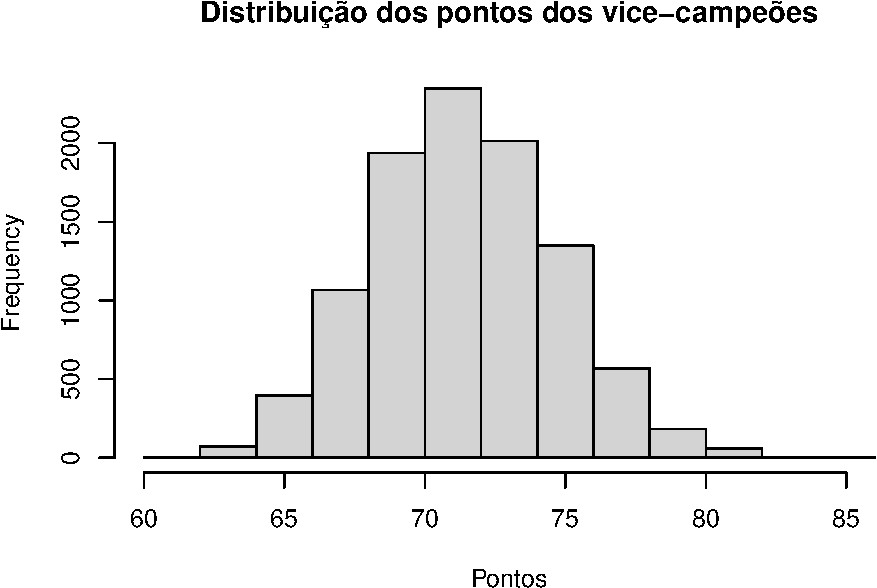
\includegraphics{trabalho1_files/trabalho1_files/figure-latex/perg5-1.pdf}

Assim, precisamos extrair o quantil 0.9, usando a função
\(\texttt{quantile()}\):

\begin{Shaded}
\begin{Highlighting}[]
\FunctionTok{quantile}\NormalTok{(}\FunctionTok{lapply}\NormalTok{(resultados, }\ControlFlowTok{function}\NormalTok{(x) \{x}\SpecialCharTok{$}\NormalTok{pontos\_todos[}\DecValTok{2}\NormalTok{, }\DecValTok{2}\NormalTok{]\}) }\SpecialCharTok{\%\textgreater{}\%}
         \FunctionTok{unlist}\NormalTok{(), }\FloatTok{0.9}\NormalTok{)}
\end{Highlighting}
\end{Shaded}

\begin{verbatim}
## 90% 
##  76
\end{verbatim}

\newpage

\hypertarget{quantos-pontos-suxe3o-necessuxe1rios-que-um-time-qualquer-fauxe7a-para-ter-pelo-menos-95-de-chance-de-nuxe3o-ser-rebaixado}{%
\subsection{6. Quantos pontos são necessários que um time qualquer faça
para ter pelo menos 95\% de chance de não ser
rebaixado?}\label{quantos-pontos-suxe3o-necessuxe1rios-que-um-time-qualquer-fauxe7a-para-ter-pelo-menos-95-de-chance-de-nuxe3o-ser-rebaixado}}

Semelhante ao caso anterior, vejamos como se comporta a pontuação do 17º
colocado na tabela (visto que é ele o time que foi rebaixado com maior
pontuação):

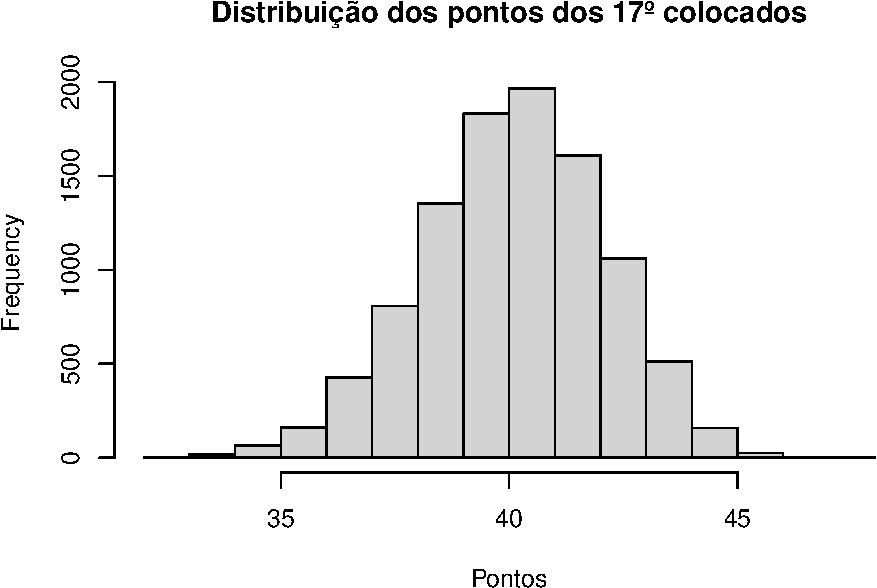
\includegraphics{trabalho1_files/trabalho1_files/figure-latex/perg6-1.pdf}

Assim, precisamos extrair o quantil 0.95, usando a função
\(\texttt{quantile()}\):

\begin{Shaded}
\begin{Highlighting}[]
\FunctionTok{quantile}\NormalTok{(}\FunctionTok{lapply}\NormalTok{(resultados, }\ControlFlowTok{function}\NormalTok{(x) \{x}\SpecialCharTok{$}\NormalTok{pontos\_todos[}\DecValTok{17}\NormalTok{, }\DecValTok{2}\NormalTok{]\}) }\SpecialCharTok{\%\textgreater{}\%}
    \FunctionTok{unlist}\NormalTok{(), }\FloatTok{0.95}\NormalTok{)}
\end{Highlighting}
\end{Shaded}

\begin{verbatim}
## 95% 
##  44
\end{verbatim}

\newpage

\hypertarget{bootstrap}{%
\section{Bootstrap}\label{bootstrap}}

Se quisermos avaliar a variabilidade inerente para os \(\theta\)'s e
\(\phi\)'s, podemos fazer um estudo de reamostragem por bootstrap, e
recalcular esses valores uma quantidade suficientemente grande de vezes.

\begin{Shaded}
\begin{Highlighting}[]
\CommentTok{\# Número de amostras bootstrap:}
\NormalTok{B }\OtherTok{\textless{}{-}} \DecValTok{1000}

\CommentTok{\# Matrizes com os valores de cada estimativa:}
\NormalTok{boot\_theta\_m }\OtherTok{\textless{}{-}} \FunctionTok{matrix}\NormalTok{(}\ConstantTok{NA}\NormalTok{, }\AttributeTok{nrow =}\NormalTok{ B,}
                       \AttributeTok{ncol =} \FunctionTok{length}\NormalTok{(}\FunctionTok{unique}\NormalTok{(jogos\_realizados}\SpecialCharTok{$}\NormalTok{time\_mandante)),}
                       \AttributeTok{dimnames =} \FunctionTok{list}\NormalTok{(}\ConstantTok{NULL}\NormalTok{,}
                                       \FunctionTok{unique}\NormalTok{(jogos\_realizados}\SpecialCharTok{$}\NormalTok{time\_mandante) }\SpecialCharTok{\%\textgreater{}\%} \FunctionTok{sort}\NormalTok{()))}
\NormalTok{boot\_theta\_v }\OtherTok{\textless{}{-}} \FunctionTok{matrix}\NormalTok{(}\ConstantTok{NA}\NormalTok{, }\AttributeTok{nrow =}\NormalTok{ B,}
                       \AttributeTok{ncol =} \FunctionTok{length}\NormalTok{(}\FunctionTok{unique}\NormalTok{(jogos\_realizados}\SpecialCharTok{$}\NormalTok{time\_mandante)),}
                       \AttributeTok{dimnames =} \FunctionTok{list}\NormalTok{(}\ConstantTok{NULL}\NormalTok{,}
                                       \FunctionTok{unique}\NormalTok{(jogos\_realizados}\SpecialCharTok{$}\NormalTok{time\_mandante) }\SpecialCharTok{\%\textgreater{}\%} \FunctionTok{sort}\NormalTok{()))}
\NormalTok{boot\_phi\_m }\OtherTok{\textless{}{-}} \FunctionTok{matrix}\NormalTok{(}\ConstantTok{NA}\NormalTok{, }\AttributeTok{nrow =}\NormalTok{ B,}
                     \AttributeTok{ncol =} \FunctionTok{length}\NormalTok{(}\FunctionTok{unique}\NormalTok{(jogos\_realizados}\SpecialCharTok{$}\NormalTok{time\_mandante)),}
                     \AttributeTok{dimnames =} \FunctionTok{list}\NormalTok{(}\ConstantTok{NULL}\NormalTok{,}
                                     \FunctionTok{unique}\NormalTok{(jogos\_realizados}\SpecialCharTok{$}\NormalTok{time\_mandante) }\SpecialCharTok{\%\textgreater{}\%} \FunctionTok{sort}\NormalTok{()))}
\NormalTok{boot\_phi\_v }\OtherTok{\textless{}{-}} \FunctionTok{matrix}\NormalTok{(}\ConstantTok{NA}\NormalTok{, }\AttributeTok{nrow =}\NormalTok{ B,}
                     \AttributeTok{ncol =} \FunctionTok{length}\NormalTok{(}\FunctionTok{unique}\NormalTok{(jogos\_realizados}\SpecialCharTok{$}\NormalTok{time\_mandante)),}
                     \AttributeTok{dimnames =} \FunctionTok{list}\NormalTok{(}\ConstantTok{NULL}\NormalTok{,}
                                     \FunctionTok{unique}\NormalTok{(jogos\_realizados}\SpecialCharTok{$}\NormalTok{time\_mandante) }\SpecialCharTok{\%\textgreater{}\%} \FunctionTok{sort}\NormalTok{()))}

\CommentTok{\# Seed para reprodutibilidade:}
\FunctionTok{set.seed}\NormalTok{(}\DecValTok{5050}\NormalTok{)}

\CommentTok{\# Bootstrap}
\ControlFlowTok{for}\NormalTok{(i }\ControlFlowTok{in} \DecValTok{1}\SpecialCharTok{:}\NormalTok{B) \{}
    \CommentTok{\# Extrai uma amostra com reposição dos jogos realizados:}
\NormalTok{    amostra }\OtherTok{\textless{}{-}}\NormalTok{ jogos\_realizados[}\FunctionTok{sample}\NormalTok{(}\DecValTok{1}\SpecialCharTok{:}\FunctionTok{nrow}\NormalTok{(jogos\_realizados),}
                                       \AttributeTok{replace =} \ConstantTok{TRUE}\NormalTok{), ]}
    \CommentTok{\# Recalcula as taxas:}
\NormalTok{    taxas\_estimadas\_boot }\OtherTok{\textless{}{-}} \FunctionTok{left\_join}\NormalTok{(}
\NormalTok{    (amostra }\SpecialCharTok{\%\textgreater{}\%}
     \FunctionTok{mutate}\NormalTok{(}\AttributeTok{time =}\NormalTok{ time\_mandante) }\SpecialCharTok{\%\textgreater{}\%}
     \FunctionTok{group\_by}\NormalTok{(time) }\SpecialCharTok{\%\textgreater{}\%}
     \FunctionTok{summarise}\NormalTok{(}\AttributeTok{theta\_m =} \FunctionTok{mean}\NormalTok{(gols\_mandante, }\AttributeTok{na.rm =}\NormalTok{ T),}
               \AttributeTok{phi\_v =} \FunctionTok{mean}\NormalTok{(gols\_visitante, }\AttributeTok{na.rm =}\NormalTok{ T))),}
\NormalTok{    (amostra }\SpecialCharTok{\%\textgreater{}\%}
     \FunctionTok{mutate}\NormalTok{(}\AttributeTok{time =}\NormalTok{ time\_visitante) }\SpecialCharTok{\%\textgreater{}\%}
     \FunctionTok{group\_by}\NormalTok{(time) }\SpecialCharTok{\%\textgreater{}\%}
     \FunctionTok{summarise}\NormalTok{(}\AttributeTok{theta\_v =} \FunctionTok{mean}\NormalTok{(gols\_visitante, }\AttributeTok{na.rm =}\NormalTok{ T),}
               \AttributeTok{phi\_m =} \FunctionTok{mean}\NormalTok{(gols\_mandante, }\AttributeTok{na.rm =}\NormalTok{ T))), }\AttributeTok{by =} \StringTok{"time"}\NormalTok{)}
    \CommentTok{\# Aplica os valores por linha nas matrizes:}
\NormalTok{    boot\_theta\_m[i, ] }\OtherTok{\textless{}{-}}\NormalTok{ taxas\_estimadas\_boot}\SpecialCharTok{$}\NormalTok{theta\_m}
\NormalTok{    boot\_theta\_v[i, ] }\OtherTok{\textless{}{-}}\NormalTok{ taxas\_estimadas\_boot}\SpecialCharTok{$}\NormalTok{theta\_v}
\NormalTok{    boot\_phi\_m[i, ] }\OtherTok{\textless{}{-}}\NormalTok{ taxas\_estimadas\_boot}\SpecialCharTok{$}\NormalTok{phi\_m}
\NormalTok{    boot\_phi\_v[i, ] }\OtherTok{\textless{}{-}}\NormalTok{ taxas\_estimadas\_boot}\SpecialCharTok{$}\NormalTok{phi\_v}
\NormalTok{\}}
\end{Highlighting}
\end{Shaded}

Com isso, podemos construir boxplots para cada uma das taxas estimadas,
considerando cada time. Neles, teremos ideia da variabilidade por meio
do intervalo interquantílico e mediana das reamostras bootstrap. Além
disso, o valor original será colocado como um ponto vermelho, para
título de comparação.

\begin{center}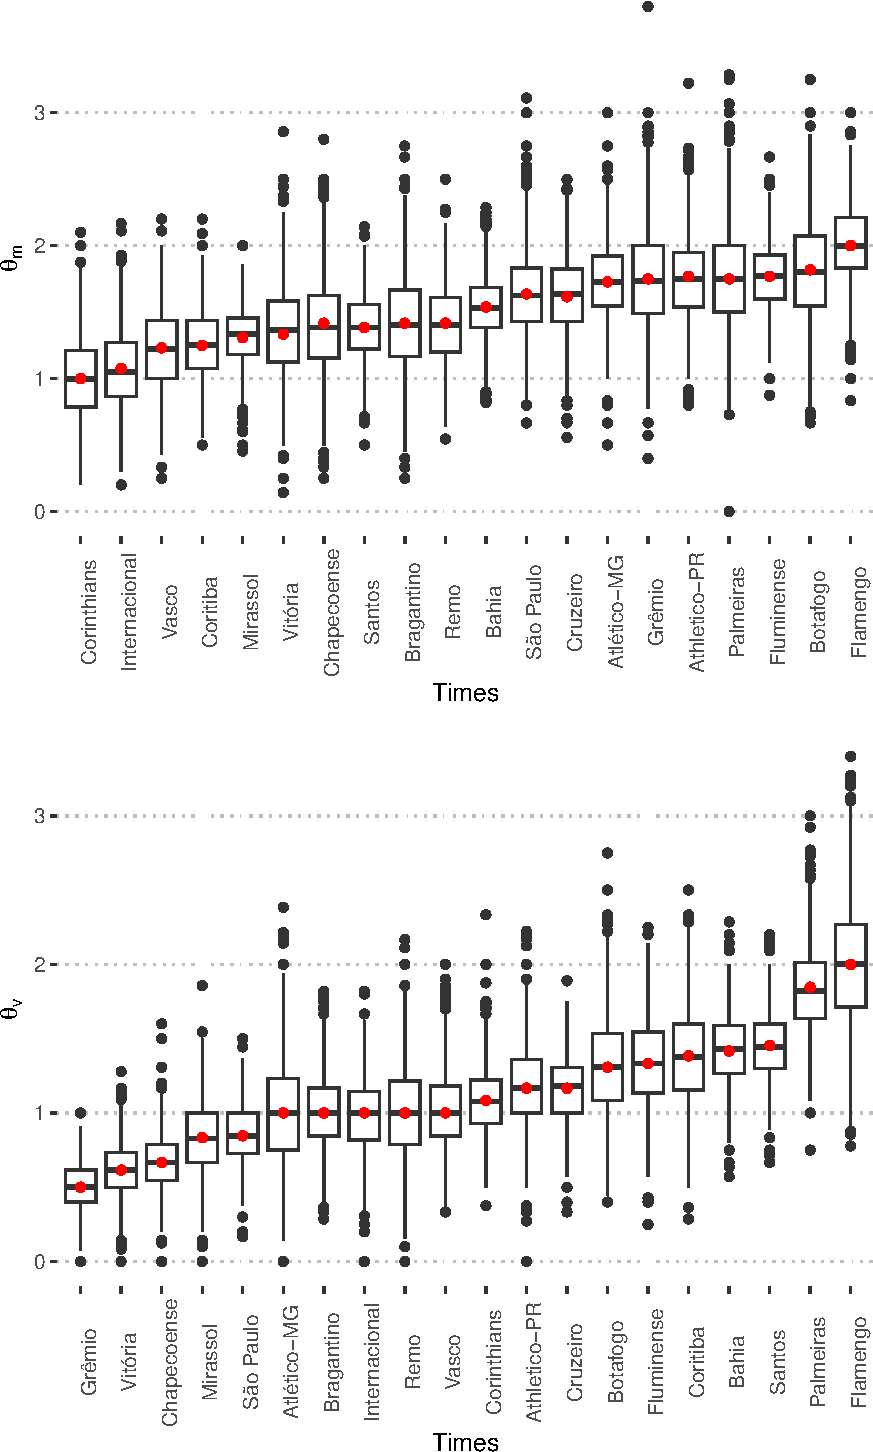
\includegraphics{trabalho1_files/figure-latex/graf_bootstrap1-1} \end{center}

\newpage

\begin{center}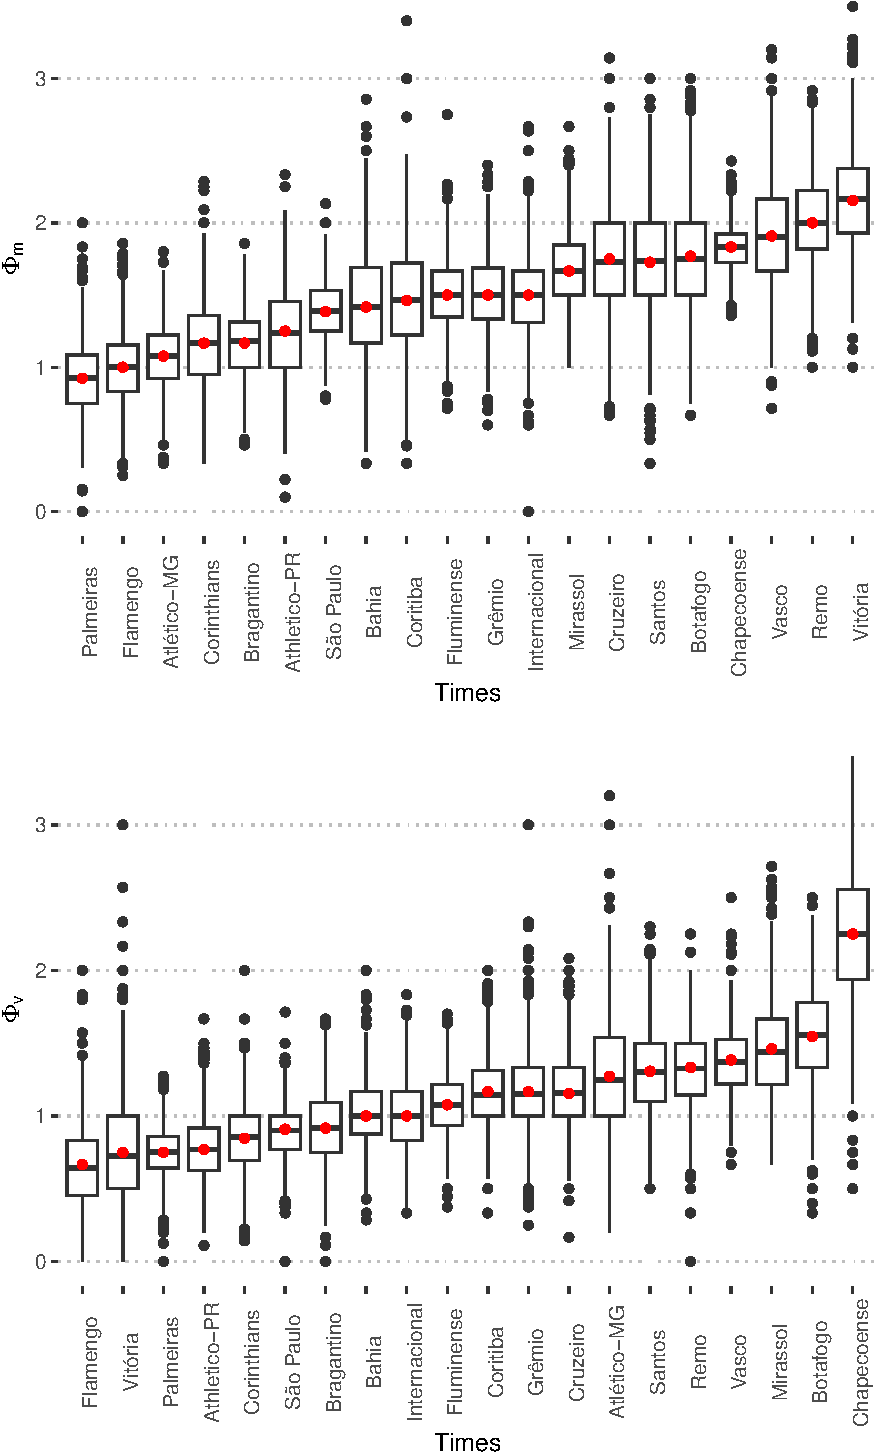
\includegraphics{trabalho1_files/figure-latex/graf_bootstrap2-1} \end{center}

\hypertarget{atividade-extra}{%
\section{Atividade Extra}\label{atividade-extra}}

Uma maneira de aprimorar as estimativas, seria por meio de uma taxa para
simulação que não seja fixa, mas que se adapte conforme o campeonato
evolui. Para isso, o mais usual é utilizar uma média móvel, com uma
janela fixa (por exemplo, considerar a média das \(k\) últimas
partidas), porém essa abordagem desconsidera os jogos mais antigos, em
favor dos novos.

Uma maneira de mitigar isso, é por meio de Médias Móveis
Exponencialmente Ponderadas (\emph{Exponentially Weighted Moving
Averages}, ou \textbf{EWMA}), que considera todas as partidas
anteriores, com pesos que decaem de maneira exponencial. Assim,
pondera-se o último jogo com mais importância, mas sem descartar os
jogos passados.

\begin{Shaded}
\begin{Highlighting}[]
\CommentTok{\# O parâmetro alpha controla o "esquecimento" do modelo,}
\CommentTok{\# alpha = 0.2 significa que o jogo atual tem 20\% de peso}
\CommentTok{\# na nova taxa, e o histórico 80\%:}
\NormalTok{alpha }\OtherTok{\textless{}{-}} \FloatTok{0.20}

\NormalTok{calcula\_ewma }\OtherTok{\textless{}{-}} \ControlFlowTok{function}\NormalTok{(vetor\_gols) \{}
    \FunctionTok{accumulate}\NormalTok{(vetor\_gols, }\SpecialCharTok{\textasciitilde{}}\NormalTok{ alpha }\SpecialCharTok{*}\NormalTok{ .y }\SpecialCharTok{+}\NormalTok{ (}\DecValTok{1} \SpecialCharTok{{-}}\NormalTok{ alpha) }\SpecialCharTok{*}\NormalTok{ .x,}
               \AttributeTok{.init =}\NormalTok{ vetor\_gols[}\DecValTok{1}\NormalTok{])[}\SpecialCharTok{{-}}\DecValTok{1}\NormalTok{]}
\NormalTok{\}}

\CommentTok{\# Criamos o histórico de maneira linear, pois agora}
\CommentTok{\# não há mais importância se o time atuou como mandante}
\CommentTok{\# ou visitante em cada partida:}
\NormalTok{taxas\_finais\_ewma }\OtherTok{\textless{}{-}}\NormalTok{ jogos\_realizados }\SpecialCharTok{\%\textgreater{}\%}
    \FunctionTok{pivot\_longer}\NormalTok{(}
        \AttributeTok{cols =} \FunctionTok{c}\NormalTok{(time\_mandante, time\_visitante),}
        \AttributeTok{names\_to =} \StringTok{"mando"}\NormalTok{,}
        \AttributeTok{values\_to =} \StringTok{"time"}
\NormalTok{    ) }\SpecialCharTok{\%\textgreater{}\%}
    \FunctionTok{mutate}\NormalTok{(}
        \AttributeTok{gols\_feitos =} \FunctionTok{ifelse}\NormalTok{(mando }\SpecialCharTok{==} \StringTok{"time\_mandante"}\NormalTok{,}
\NormalTok{                             gols\_mandante, gols\_visitante),}
        \AttributeTok{gols\_sofridos =} \FunctionTok{ifelse}\NormalTok{(mando }\SpecialCharTok{==} \StringTok{"time\_mandante"}\NormalTok{,}
\NormalTok{                               gols\_visitante, gols\_mandante)}
\NormalTok{    ) }\SpecialCharTok{\%\textgreater{}\%}
    \FunctionTok{arrange}\NormalTok{(time, rodada) }\SpecialCharTok{\%\textgreater{}\%}
    \FunctionTok{group\_by}\NormalTok{(time) }\SpecialCharTok{\%\textgreater{}\%}
    \FunctionTok{mutate}\NormalTok{(}
        \AttributeTok{theta\_hist =} \FunctionTok{calcula\_ewma}\NormalTok{(gols\_feitos),}
        \AttributeTok{phi\_hist =} \FunctionTok{calcula\_ewma}\NormalTok{(gols\_sofridos)}
\NormalTok{    ) }\SpecialCharTok{\%\textgreater{}\%}
    \CommentTok{\# Pegamos apenas o valor da taxa na última rodada jogada}
    \CommentTok{\# pelo time para projetar o futuro:}
    \FunctionTok{slice\_tail}\NormalTok{(}\AttributeTok{n =} \DecValTok{1}\NormalTok{) }\SpecialCharTok{\%\textgreater{}\%}
    \FunctionTok{select}\NormalTok{(time, }\AttributeTok{theta\_ewma =}\NormalTok{ theta\_hist, }\AttributeTok{phi\_ewma =}\NormalTok{ phi\_hist) }\SpecialCharTok{\%\textgreater{}\%}
    \FunctionTok{ungroup}\NormalTok{()}

\NormalTok{taxas\_finais\_ewma }\SpecialCharTok{\%\textgreater{}\%}
    \FunctionTok{kable}\NormalTok{()}
\end{Highlighting}
\end{Shaded}

\begin{longtable}[]{@{}lrr@{}}
\toprule\noalign{}
time & theta\_ewma & phi\_ewma \\
\midrule\noalign{}
\endhead
\bottomrule\noalign{}
\endlastfoot
Athletico-PR & 1.8912053 & 1.2570595 \\
Atlético-MG & 1.5353075 & 0.8283330 \\
Bahia & 1.7573311 & 1.2472952 \\
Botafogo & 1.0754578 & 1.7652459 \\
Bragantino & 1.0643867 & 1.0289341 \\
Chapecoense & 1.2415546 & 2.1138784 \\
Corinthians & 1.0209123 & 1.0885315 \\
Coritiba & 1.6166863 & 1.3993980 \\
Cruzeiro & 1.5614808 & 1.3671750 \\
Flamengo & 2.3272617 & 0.8066487 \\
Fluminense & 1.7950529 & 1.5081735 \\
Grêmio & 1.2273003 & 1.4424965 \\
Internacional & 0.9608387 & 1.3846542 \\
Mirassol & 1.1022806 & 1.7637946 \\
Palmeiras & 1.9450405 & 1.0278257 \\
Remo & 1.3750885 & 1.8520406 \\
Santos & 1.4190320 & 1.1115452 \\
São Paulo & 1.0553825 & 1.2771787 \\
Vasco & 1.0506111 & 1.8414949 \\
Vitória & 0.6641979 & 1.7067209 \\
\end{longtable}

\begin{Shaded}
\begin{Highlighting}[]
\CommentTok{\# Juntamos as taxas atualizadas com a tabela}
\CommentTok{\# de jogos ainda não realizados:}
\NormalTok{jogos\_futuros\_ewma }\OtherTok{\textless{}{-}}\NormalTok{ jogos\_futuros }\SpecialCharTok{\%\textgreater{}\%}
    \FunctionTok{select}\NormalTok{(}\SpecialCharTok{{-}}\FunctionTok{c}\NormalTok{(theta\_m, theta\_v, phi\_m, phi\_v)) }\SpecialCharTok{\%\textgreater{}\%}
    \FunctionTok{left\_join}\NormalTok{(}
\NormalTok{        taxas\_finais\_ewma }\SpecialCharTok{\%\textgreater{}\%} \FunctionTok{rename}\NormalTok{(}\AttributeTok{time\_mandante =}\NormalTok{ time,}
                                     \AttributeTok{theta\_m =}\NormalTok{ theta\_ewma,}
                                     \AttributeTok{phi\_m =}\NormalTok{ phi\_ewma),}
        \AttributeTok{by =} \StringTok{"time\_mandante"}
\NormalTok{    ) }\SpecialCharTok{\%\textgreater{}\%}
    \FunctionTok{left\_join}\NormalTok{(}
\NormalTok{        taxas\_finais\_ewma }\SpecialCharTok{\%\textgreater{}\%} \FunctionTok{rename}\NormalTok{(}\AttributeTok{time\_visitante =}\NormalTok{ time,}
                                     \AttributeTok{theta\_v =}\NormalTok{ theta\_ewma,}
                                     \AttributeTok{phi\_v =}\NormalTok{ phi\_ewma),}
        \AttributeTok{by =} \StringTok{"time\_visitante"}
\NormalTok{    )}

\CommentTok{\# Para simular, usamos um esquema semelhante ao anterior,}
\CommentTok{\# porém com as taxas adaptativas:}
\NormalTok{simula\_campeonato\_ewma }\OtherTok{\textless{}{-}} \ControlFlowTok{function}\NormalTok{(...) \{}
\NormalTok{  sim\_futuros }\OtherTok{\textless{}{-}}\NormalTok{ jogos\_futuros\_ewma }\SpecialCharTok{\%\textgreater{}\%}
    \FunctionTok{mutate}\NormalTok{(}
        \AttributeTok{gols\_mandante =} \FunctionTok{rpois}\NormalTok{(}\FunctionTok{n}\NormalTok{(), (theta\_m }\SpecialCharTok{+}\NormalTok{ phi\_v)}\SpecialCharTok{/}\DecValTok{2}\NormalTok{),}
        \AttributeTok{gols\_visitante =} \FunctionTok{rpois}\NormalTok{(}\FunctionTok{n}\NormalTok{(), (theta\_v }\SpecialCharTok{+}\NormalTok{ phi\_m)}\SpecialCharTok{/}\DecValTok{2}\NormalTok{)}
\NormalTok{    )}
\NormalTok{  tabela\_simulada }\OtherTok{\textless{}{-}} \FunctionTok{calcula\_tabela}\NormalTok{(sim\_futuros)}
  \CommentTok{\# Junta o passado real com o futuro simulado e aplica os critérios de desempate}
\NormalTok{  tabela\_final }\OtherTok{\textless{}{-}} \FunctionTok{bind\_rows}\NormalTok{(tabela\_base, tabela\_simulada) }\SpecialCharTok{\%\textgreater{}\%}
      \FunctionTok{group\_by}\NormalTok{(time) }\SpecialCharTok{\%\textgreater{}\%}
      \FunctionTok{summarise}\NormalTok{(}\FunctionTok{across}\NormalTok{(}\FunctionTok{everything}\NormalTok{(), sum), }\AttributeTok{.groups =} \StringTok{"drop"}\NormalTok{) }\SpecialCharTok{\%\textgreater{}\%}
      \FunctionTok{arrange}\NormalTok{(}\FunctionTok{desc}\NormalTok{(pontos), }\FunctionTok{desc}\NormalTok{(vitorias), }\FunctionTok{desc}\NormalTok{(saldo), }\FunctionTok{desc}\NormalTok{(gols\_pro)) }\SpecialCharTok{\%\textgreater{}\%}
      \FunctionTok{mutate}\NormalTok{(}\AttributeTok{posicao =} \FunctionTok{row\_number}\NormalTok{())}
  \FunctionTok{list}\NormalTok{(}
      \AttributeTok{campeao =}\NormalTok{ tabela\_final}\SpecialCharTok{$}\NormalTok{time[}\DecValTok{1}\NormalTok{],}
      \AttributeTok{pontos\_campeao =}\NormalTok{ tabela\_final}\SpecialCharTok{$}\NormalTok{pontos[}\DecValTok{1}\NormalTok{],}
      \AttributeTok{vice =}\NormalTok{ tabela\_final}\SpecialCharTok{$}\NormalTok{time[}\DecValTok{2}\NormalTok{],}
      \AttributeTok{pontos\_vice =}\NormalTok{ tabela\_final}\SpecialCharTok{$}\NormalTok{pontos[}\DecValTok{2}\NormalTok{],}
      \AttributeTok{rebaixados =}\NormalTok{ tabela\_final}\SpecialCharTok{$}\NormalTok{time[}\DecValTok{17}\SpecialCharTok{:}\DecValTok{20}\NormalTok{],}
      \AttributeTok{pontos\_todos =}\NormalTok{ tabela\_final }\SpecialCharTok{\%\textgreater{}\%} \FunctionTok{select}\NormalTok{(time, pontos, posicao)}
\NormalTok{  )}
\NormalTok{\}}
\end{Highlighting}
\end{Shaded}

Para ver como se comportariam as taxas adaptativas, rodemos uma
simulação considerando os times paranaenses no campeonato:

\newpage

\begin{center}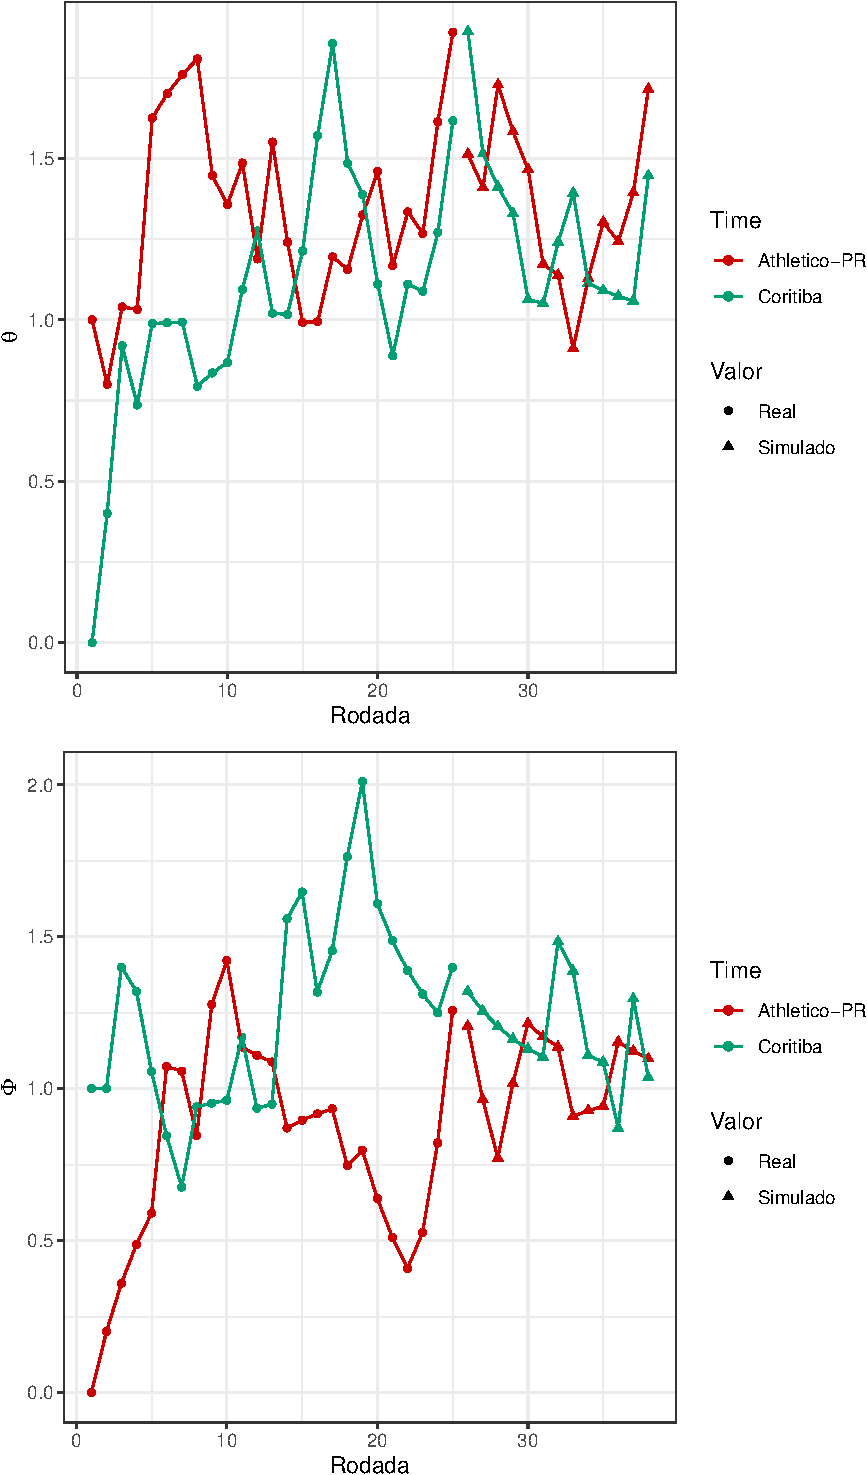
\includegraphics{trabalho1_files/figure-latex/simula_times_pr-1} \end{center}

Com isso, realizemos a simulação uma quantidade grande de vezes,
considerando agora a taxa adaptativa, e comparemos os resultados
obtidos:

\begin{Shaded}
\begin{Highlighting}[]
\NormalTok{resultados\_mc }\OtherTok{\textless{}{-}} \FunctionTok{mclapply}\NormalTok{(}\DecValTok{1}\SpecialCharTok{:}\NormalTok{n\_simulacoes, simula\_campeonato\_ewma,}
                          \AttributeTok{mc.cores =} \FunctionTok{detectCores}\NormalTok{() }\SpecialCharTok{{-}} \DecValTok{2}\NormalTok{)}
\end{Highlighting}
\end{Shaded}

\hypertarget{qual-a-probabilidade-de-cada-time-ser-campeuxe3o-1}{%
\subsection{1. Qual a probabilidade de cada time ser
campeão?}\label{qual-a-probabilidade-de-cada-time-ser-campeuxe3o-1}}

\begin{verbatim}
## Joining with `by = join_by(Time)`
\end{verbatim}

\begin{longtable}[]{@{}lll@{}}
\toprule\noalign{}
Time & Freq\_Ori & Freq\_Adap \\
\midrule\noalign{}
\endhead
\bottomrule\noalign{}
\endlastfoot
Flamengo & 57.92\% & 58.0370\% \\
Palmeiras & 38.76\% & 37.8750\% \\
Athletico-PR & 2.85\% & 3.4030\% \\
Fluminense & 0.30\% & 0.3700\% \\
Bahia & 0.09\% & 0.1170\% \\
Atlético-MG & 0.02\% & 0.1120\% \\
Cruzeiro & 0.03\% & 0.0610\% \\
Bragantino & 0.02\% & 0.0130\% \\
Coritiba & 0.01\% & 0.0120\% \\
Botafogo & 0.00\% & 0.0000\% \\
Chapecoense & 0.00\% & 0.0000\% \\
Corinthians & 0.00\% & 0.0000\% \\
Grêmio & 0.00\% & 0.0000\% \\
Internacional & 0.00\% & 0.0000\% \\
Mirassol & 0.00\% & 0.0000\% \\
Remo & 0.00\% & 0.0000\% \\
Santos & 0.00\% & 0.0000\% \\
São Paulo & 0.00\% & 0.0000\% \\
Vasco & 0.00\% & 0.0000\% \\
Vitória & 0.00\% & 0.0000\% \\
\end{longtable}

\newpage

\hypertarget{qual-a-probabilidade-de-cada-time-ser-rebaixado-1}{%
\subsection{2. Qual a probabilidade de cada time ser
rebaixado?}\label{qual-a-probabilidade-de-cada-time-ser-rebaixado-1}}

\begin{verbatim}
## Joining with `by = join_by(Time)`
\end{verbatim}

\begin{longtable}[]{@{}lll@{}}
\toprule\noalign{}
Time & Freq\_Ori & Freq\_Adap \\
\midrule\noalign{}
\endhead
\bottomrule\noalign{}
\endlastfoot
Chapecoense & 24.8575\% & 24.72675\% \\
Remo & 18.5350\% & 17.95425\% \\
Mirassol & 15.1250\% & 14.14600\% \\
Vasco & 14.7675\% & 13.32900\% \\
Internacional & 12.2175\% & 10.95950\% \\
Vitória & 4.5425\% & 8.75850\% \\
Grêmio & 4.2050\% & 3.51550\% \\
Botafogo & 0.9200\% & 3.10675\% \\
São Paulo & 1.2225\% & 1.51850\% \\
Santos & 2.7100\% & 1.18950\% \\
Corinthians & 0.6900\% & 0.70475\% \\
Bragantino & 0.0525\% & 0.05175\% \\
Coritiba & 0.1000\% & 0.02975\% \\
Atlético-MG & 0.0300\% & 0.00400\% \\
Cruzeiro & 0.0200\% & 0.00375\% \\
Bahia & 0.0050\% & 0.00125\% \\
Fluminense & 0.0000\% & 0.00050\% \\
Athletico-PR & 0.0000\% & 0.00000\% \\
Flamengo & 0.0000\% & 0.00000\% \\
Palmeiras & 0.0000\% & 0.00000\% \\
\end{longtable}

\newpage

\hypertarget{qual-a-probabilidade-do-campeonato-ser-decidido-pelos-crituxe9rios-de-desempate-1}{%
\subsection{3. Qual a probabilidade do campeonato ser decidido pelos
critérios de
desempate?}\label{qual-a-probabilidade-do-campeonato-ser-decidido-pelos-crituxe9rios-de-desempate-1}}

\begin{verbatim}
## [1] "Original:"
\end{verbatim}

\begin{verbatim}
## [1] "6.34%"
\end{verbatim}

\begin{verbatim}
## [1] "Adaptativo:"
\end{verbatim}

\begin{verbatim}
## [1] "6.53%"
\end{verbatim}

\hypertarget{qual-o-valor-esperado-do-nuxfamero-de-pontos-do-campeuxe3o-1}{%
\subsection{4. Qual o valor esperado do número de pontos do
campeão?}\label{qual-o-valor-esperado-do-nuxfamero-de-pontos-do-campeuxe3o-1}}

\begin{verbatim}
## [1] "Original:"
\end{verbatim}

\begin{verbatim}
## [1] 76.974
\end{verbatim}

\begin{verbatim}
## [1] "Adaptativo:"
\end{verbatim}

\begin{verbatim}
## [1] 77.2113
\end{verbatim}

\newpage

\hypertarget{quantos-pontos-uma-qualquer-equipe-precisa-fazer-para-ter-pelo-menos-90-de-chance-de-ser-o-campeuxe3o-1}{%
\subsection{5. Quantos pontos uma qualquer equipe precisa fazer para ter
pelo menos 90\% de chance de ser o
campeão?}\label{quantos-pontos-uma-qualquer-equipe-precisa-fazer-para-ter-pelo-menos-90-de-chance-de-ser-o-campeuxe3o-1}}

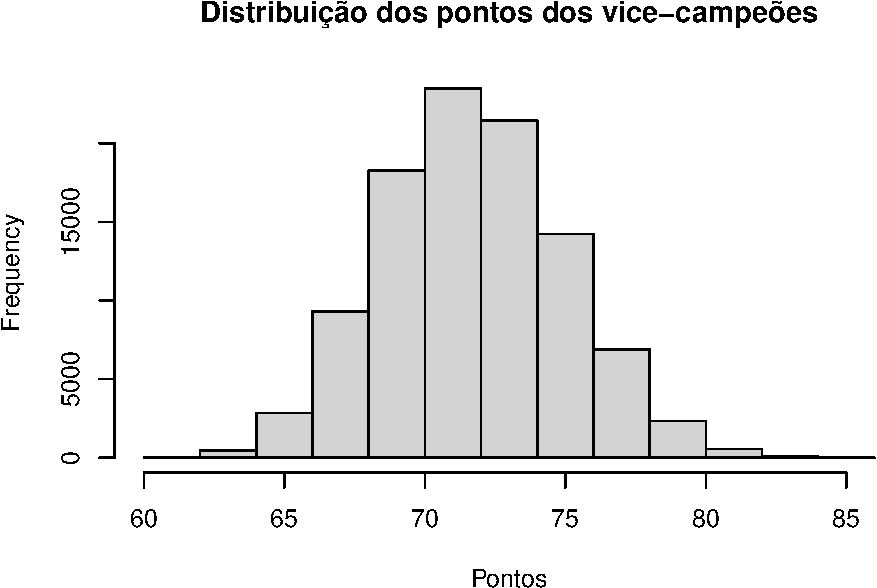
\includegraphics{trabalho1_files/trabalho1_files/figure-latex/perg5_comp-1.pdf}

\begin{verbatim}
## [1] "Original:"
\end{verbatim}

\begin{verbatim}
## 90% 
##  76
\end{verbatim}

\begin{verbatim}
## [1] "Adaptativo:"
\end{verbatim}

\begin{verbatim}
## 90% 
##  76
\end{verbatim}

\newpage

\hypertarget{quantos-pontos-suxe3o-necessuxe1rios-que-um-time-qualquer-fauxe7a-para-ter-pelo-menos-95-de-chance-de-nuxe3o-ser-rebaixado-1}{%
\subsection{6. Quantos pontos são necessários que um time qualquer faça
para ter pelo menos 95\% de chance de não ser
rebaixado?}\label{quantos-pontos-suxe3o-necessuxe1rios-que-um-time-qualquer-fauxe7a-para-ter-pelo-menos-95-de-chance-de-nuxe3o-ser-rebaixado-1}}

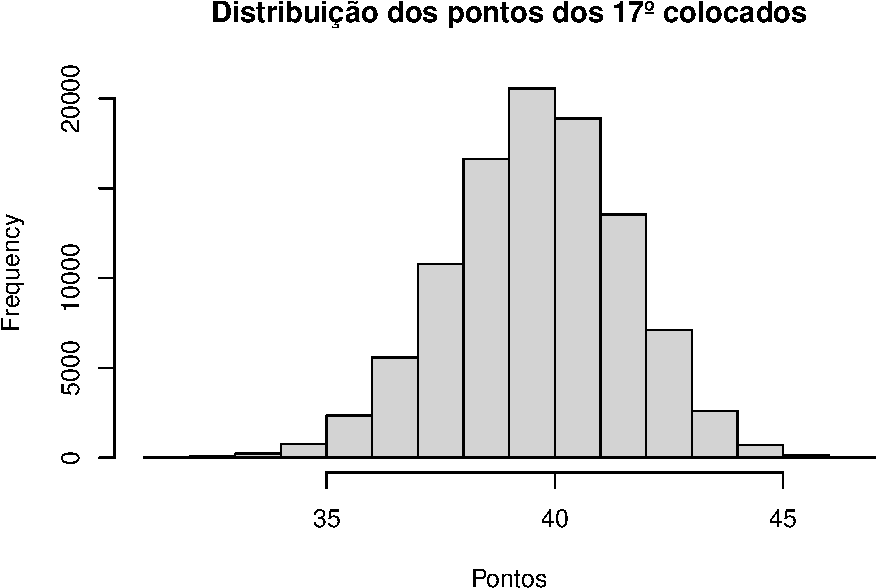
\includegraphics{trabalho1_files/trabalho1_files/figure-latex/perg6_comp-1.pdf}

\begin{verbatim}
## [1] "Original:"
\end{verbatim}

\begin{verbatim}
## 95% 
##  44
\end{verbatim}

\begin{verbatim}
## [1] "Adaptativo:"
\end{verbatim}

\begin{verbatim}
## 95% 
##  43
\end{verbatim}





\newpage
\singlespacing
\end{document}
